\documentclass[a4paper, fleqn]{article}
\usepackage{header}

\title{Семинарский лист 2.5}
\author{
    % Александр Богданов   \\ \href{https://t.me/SphericalPotatoInVacuum}{Telegram} \and
    % Алиса Вернигор       \\ \href{https://t.me/allisyonok}{Telegram} \and
    % Анастасия Григорьева \\ \href{https://t.me/weifoll}{Telegram} \and
    % Василий Шныпко       \\ \href{https://t.me/yourvash}{Telegram} \and
    % Данил Казанцев       \\ \href{https://t.me/vserosbuybuy}{Telegram} \and
    % Денис Козлов         \\ \href{https://t.me/DKozl50}{Telegram} \and
    % Елизавета Орешонок   \\ \href{https://t.me/eaoresh}{Telegram} \and
    % Ира Голобородько     \\ \href{https://t.me/Ira4kgl}{Telegram} \and
    % Иван Пешехонов       \\ \href{https://t.me/JohanDDC}{Telegram} \and
    % Иван Добросовестнов  \\ \href{https://t.me/ivankot13}{Telegram} \and
    % Настя Городилова     \\ \href{https://t.me/nastygorodi}{Telegram} \and
    % Никита Насонков      \\ \href{https://t.me/nnv_nick}{Telegram} \and
    % Сергей Лоптев        \\ \href{https://t.me/beast_sl}{Telegram}
}

\date{Версия от {\ddmmyyyydate\today} \currenttime}

\begin{document}
    \maketitle
    
    \section*{Задайте в полярных координатах множество $D$, заданное неравенствами в декартовых координатах.
    Предполагая функцию $f$ непрерывной на $D$, преобразуйте интеграл в полярных координатах к повторному.}
    \subsection*{Задача 1}
    \begin{flalign*}
        & x^2+y^2 \le 2x \\[5 pt]
        & x = r \cos \varphi, \; y = r \sin \varphi \Rightarrow \\
        & \Rightarrow  D := r^2 \le 2\, r \cos \varphi \Leftrightarrow r (r - 2 \cos \varphi) \le 0 
        \Leftrightarrow r \in \left[0; 2 \cos \varphi\right], \cos \varphi \ge 0 \\
        & \iint\limits_D f(r \cos \varphi, r \sin \varphi)\, d\varphi\,dr
        = \int\limits_{-\pi/2}^{\pi/2} d\varphi \int\limits_{0}^{2 \cos \varphi} f(r \cos \varphi, r \sin \varphi)\, r \,dr = \\
        & \left\{\, r^2 \le 2\, r \cos \varphi \Leftrightarrow \cos \varphi \ge \frac{r}2 
        \Leftrightarrow \varphi \in \left[ -\arccos \frac{r}2; \arccos \frac{r}2 \right] \,\right\} \\
        & = \int\limits_{0}^{2} r\, dr \int\limits_{-\arccos \frac{r}2}^{\arccos \frac{r}2} f(r \cos \varphi, r \sin \varphi)\, d\varphi 
    \end{flalign*}
    
    \subsection*{Задача 2}
    \begin{flalign*}
        & (x-1)^2+y^2 \le 1, \; x^2 + y^2 \ge 1 \\[5 pt]
        & x = r \cos \varphi, \; y = r \sin \varphi \Rightarrow \\
        & \Rightarrow  D := \left\{\begin{array}{lll} r^2 &\le& 2\,r \cos \varphi, \\ r^2 &\ge& 1 \end{array}\right. 
        \Leftrightarrow \left\{\begin{array}{rcl} 
            r &\in& \left[ 0; 2 \cos \varphi \right], \\  
            \cos \varphi &\ge& 0, \\ 
            r &\ge& 1 
        \end{array}\right. \Leftrightarrow \left\{\begin{array}{rcl} 
            r &\in& \left[ 1; 2 \cos \varphi \right], \\  
            \cos \varphi &\ge& 1/2, \\ 
        \end{array}\right. \\
        & \cos \varphi \ge 1/2 \Leftrightarrow \varphi \in \left[ -\dfrac{\pi}3; \dfrac{\pi}3 \right] \\
        & \iint\limits_D f(r \cos \varphi, r \sin \varphi)\, d\varphi\,dr
        = \int\limits_{-\pi/3}^{\pi/3} d\varphi \int\limits_{1}^{2 \cos \varphi} f(r \cos \varphi, r \sin \varphi)\, r \,dr = \\
        & \left\{\, r^2 \le 2\,r \cos \varphi \Leftrightarrow \cos \varphi \ge \frac{r}2 
        \Leftrightarrow \varphi \in \left[ -\arccos \frac{r}2; \arccos \frac{r}2 \right] \,\right\} \\
        & = \int\limits_{1}^{2} r\, dr \int\limits_{-\arccos \frac{r}2}^{\arccos \frac{r}2} f(r \cos \varphi, r \sin \varphi)\, d\varphi 
    \end{flalign*}
    
    % \subsection*{Задача 3}
    
    \subsection*{Задача 4}
    \begin{wrapfigure}{r}{0.4\textwidth}
    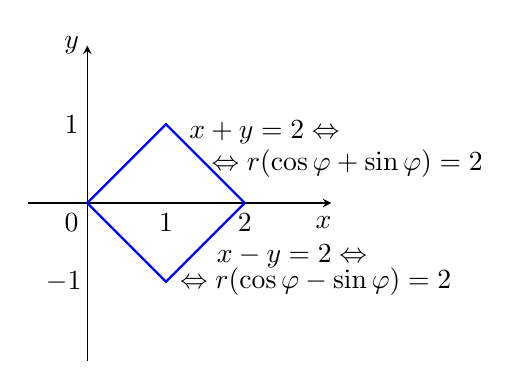
\begin{tikzpicture}[>=stealth]
       % \draw[very thick, blue, fill=pink]
        %(-3,0) -- (-1,0) -- (0,1) -- (1,0) -- (3,0) -- (0,3) -- cycle;
        %\draw[very thick, blue, fill=magenta]
        %(-3,0) -- (-1,0) -- (-0.5,0.5) -- (-0.5,2.5) -- cycle;
        \draw[->] (-0.75,0) -- (3.1,0); % Ох
        \draw[->] (0,-2) -- (0,2); % Оу
        \node at (-0.2,-0.25) {\color{black} $0$};
        \node at (3,-0.25) {\color{black} $x$};
        \node at (-0.2,2) {\color{black} $y$};
        \node at (1,-0.25) {\color{black} $1$};
        \node at (2,-0.25) {\color{black} $2$};
        \node at (-0.2,1) {\color{black} $1$};
        \node at (-0.3,-1) {\color{black} $-1$};
        \node at (2.25,0.9) {\color{black} $x+y=2 \Leftrightarrow$};
        \node at (3.3,0.5) {\color{black} $\Leftrightarrow r (\cos \varphi+\sin \varphi)=2$};
        \node at (2.6,-0.67) {\color{black} $x-y=2 \Leftrightarrow$};
        \node at (2.9,-1) {\color{black} $\Leftrightarrow r (\cos \varphi-\sin \varphi)=2$};
        \draw[thick, blue, domain=0:2] plot (\x, {abs(\x-1)-1});
        \draw[thick, blue, domain=0:2] plot (\x, {1-abs(\x-1)});
    \end{tikzpicture}
    \end{wrapfigure}
    \begin{flalign*}
        & |x-1| + |y| \le 1 \\[5 pt]
        & \text{Область представляет собой ромб с центром в точке $(1, 0)$} \\
        & \text{Из рисунка видно, что угол $\varphi$ лежит в пределах $\left[-\pi/4; \pi/4\right]$} \\
        & \text{Можно определить и отрезки для $r$}: \\
        & r \in \left\{\begin{array}{ll} 
            \left[ 0; \dfrac2{\cos \varphi + \sin \varphi} \right], & \varphi \ge 0 \\[10 pt]
            \left[ 0; \dfrac2{\cos \varphi - \sin \varphi} \right], & \varphi < 0  \\ 
        \end{array}\right. \\
        & \iint\limits_D f(r \cos \varphi, r \sin \varphi\, d\varphi\,dr
        = \int\limits_{-\pi/4}^{0} d\varphi \int\limits_{0}^{\frac2{\cos \varphi - \sin \varphi}} f(r \cos \varphi, r \sin \varphi)\, r \,dr + \int\limits_{0}^{\pi/4} d\varphi \int\limits_{0}^{\frac2{\cos \varphi + \sin \varphi}} f(r \cos \varphi, r \sin \varphi)\, r \,dr = \\[-10 pt]
        & = \int\limits_{-\pi/4}^{\pi/4} d\varphi \int\limits_{0}^{\frac2{\cos \varphi + |\sin \varphi|}} f(r \cos \varphi, r \sin \varphi)\, r \,dr \\
        & \text{При $r \in [0; \sqrt2]$ все углы от $-\pi/4$ до $\pi/4$ лежит в нужной области} \\[-5 pt]
        & \text{При $r \in (\sqrt2; 2 \sqrt2]$ необходимо } 2 \ge r (\cos \varphi + |\sin \varphi|) \\
        & \text{Так как относительно $Oy$ все симметрично, найдем границу при $\varphi > 0$:} \\
        & \text{из геометрии рисунка (треугольников и всего такого)} \\[-10 pt]
        & r \cos \left( \dfrac{\pi}4 - \varphi \right) = \sqrt2 
        \Leftrightarrow \cos \left( \dfrac{\pi}4 - \varphi \right) = \dfrac{\sqrt2}r
        \Leftrightarrow \varphi = \frac{\pi}4 - \arccos \dfrac{\sqrt2}{r} \\[-5 pt]
        & \text{Повторный интеграл с найденными границами:} \\[-10 pt]
        & \int\limits_{0}^{\sqrt2} r\, dr \int\limits_{-\pi/4}^{\pi/4} f(r \cos \varphi, r \sin \varphi)\, d\varphi 
        + \int\limits_{\sqrt2}^{2\sqrt2} r\, dr \int\limits_{\arccos \frac{\sqrt2}{r} - \frac{\pi}4}^{\frac{\pi}4 - \arccos \frac{r}{\sqrt2}} f(r \cos \varphi, r \sin \varphi)\, d\varphi 
    \end{flalign*}
    
    % \subsection*{Задача 5}
    
    \subsection*{Задача 6}
    $D$ --- множество, лежащее вне окружности $x^2 + y^2 = 1$ и внутри петель кривой $(x^2 + y^2)^2 = 2(x^2 - y^2)$ \\[5 pt]
    Так как область лежит вне окружности $x^2 + y^2 = 1$, в полярных координатах $r > 1$. \\[3 pt]
    Определим условия, необходимые и достаточные для того, чтобы координаты лежали внутри петель кривой: \\[3 pt]
    $(x^2 + y^2)^2 = 2\, (x^2 - y^2) \Leftrightarrow r^4 = 2\, r^2 (\cos^2 \varphi - \sin^2 \varphi)
     \Leftrightarrow r^2 = 2 \cos 2\, \varphi$ \\[5 pt]
     Тогда точка с полярными координатами $(r, \varphi)$ лежит внутри петель, если 
     $r^2 \le 2 \cos 2\, \varphi \Leftrightarrow \cos 2\, \varphi \ge \dfrac{r^2}2 \Leftrightarrow 
     \varphi \in \left[ -\dfrac12\arccos \dfrac{r^2}2; \dfrac12\arccos \dfrac{r^2}2 \right]$ \\
     Повторный интеграл:
     $\int\limits_{1}^{\sqrt2} r\, dr \int\limits_{-\frac12\arccos \frac{r^2}2}^{\frac12\arccos \frac{r^2}2} f(r \cos \varphi, r \sin \varphi)\, d\varphi$
    
    \section*{Перейдя к полярным координатам, вычислите интеграл.}
    % \subsection*{Задача 7}
    
    % \subsection*{Задача 8}
    
    \section*{Перейдите к переменным, в которых область интегрирования имеет вид прямоугольника, 
    и вычислите интеграл.}
    % \subsection*{Задача 9}
    
    % \subsection*{Задача 10}
    
    % \subsection*{Задача 11}
    
    \subsection*{Задача 12}
    \begin{wrapfigure}{r}{0.4\textwidth}
    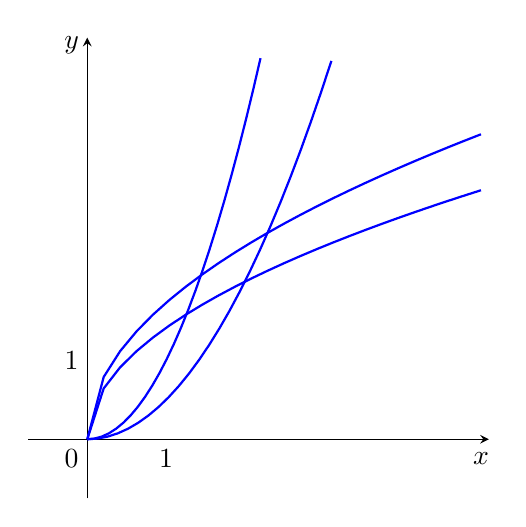
\begin{tikzpicture}[>=stealth]
        \draw[->] (-0.75,0) -- (5.1,0); % Ох
        \draw[->] (0,-0.75) -- (0,5.1); % Оу
        \node at (-0.2,-0.25) {\color{black} $0$};
        \node at (5,-0.25) {\color{black} $x$};
        \node at (-0.2,5) {\color{black} $y$};
        \node at (1,-0.25) {\color{black} $1$};
        % \node at (2,-0.25) {\color{black} $2$};
        \node at (-0.2,1) {\color{black} $1$};
        % \node at (2.25,0.9) {\color{black} $x+y=2 \Leftrightarrow$};
        % \node at (3.3,0.5) {\color{black} $\Leftrightarrow r (\cos \varphi+\sin \varphi)=2$};
        % \node at (2.6,-0.67) {\color{black} $x-y=2 \Leftrightarrow$};
        % \node at (2.9,-1) {\color{black} $\Leftrightarrow r (\cos \varphi-\sin \varphi)=2$};
        \draw[thick, blue, domain=0:2.2] plot (\x, {\x*\x});
        \draw[thick, blue, domain=0:3.1] plot (\x, {0.5*\x*\x});
        \draw[thick, blue, domain=0:5] plot (\x, {sqrt(2*\x)});
        \draw[thick, blue, domain=0:5] plot (\x, {sqrt(3*\x)});
    \end{tikzpicture}
    \end{wrapfigure}
    \begin{flalign*}
        & \iint\limits_D \dfrac{x^2 \sin (xy)}{y}\, dx\,dy, \;\;\; D = \{(x, y) \,|\, y \le x^2 \le 2y,\; 2x \le y^2 \le 3x\} \\
        & \text{Хотим, чтобы область, заданная пересечением парабол, была} \\
        & \text{прямоугольником в какой-то системе координат} \\
        & \text{Перейдем к координатам $u$ и $v$ таким, что } u = \dfrac{x^2}y, \; v = \dfrac{y^2}x. \\
        & \text{Тогда } D = \{ (u, v) \,|\, 1 \le u \le 2, \; 2 \le v \le 3 \} \\[5 pt]
        & \text{Выражение старых координат через новые:} \\[-5 pt]
        & u = \dfrac{x^2}y \Rightarrow y = \dfrac{x^2}u \Rightarrow v = \dfrac{x^4}{u^2 x} = \dfrac{x^3}{u^2}
        \Rightarrow x = \sqrt[3]{u^2 v}, \; y = \sqrt[3]{\dfrac{u^4 v^2}{u^3}} = \sqrt[3]{u v^2} \\
        & J = \left|\begin{matrix} x_u & y_u \\ x_v & y_v \end{matrix}\right| = 
        \left|\begin{matrix} \sqrt[3]{\dfrac{2v}{3u}} & \sqrt[3]{\dfrac{v^2}{3u^2}} \\[10 pt] \sqrt[3]{\dfrac{u^2}{3v^2}} & \sqrt[3]{\dfrac{2u}{3v}} \end{matrix}\right| = \sqrt[3]{\dfrac{4uv}{9uv}} - \sqrt[3]{\dfrac{u^2v^2}{9u^2v^2}} = \sqrt[3]{\dfrac{4}{9}} - \sqrt[3]{\dfrac{1}{9}} \\
        & I = \int\limits_1^2 du \int\limits_2^3 \dfrac{\sqrt[3]{u^4 v^2} \sin (uv)}{\sqrt[3]{uv^2}} \left( \sqrt[3]{\dfrac{4}{9}} - \sqrt[3]{\dfrac{1}{9}} \right) dv = 
        \left( \sqrt[3]{\dfrac{4}{9}} - \sqrt[3]{\dfrac{1}{9}} \right)\int\limits_1^2 u\, du \int\limits_2^3 \sin (uv)\, dv = \\ 
        & = \left( \sqrt[3]{\dfrac{4}{9}} - \sqrt[3]{\dfrac{1}{9}} \right)\int\limits_1^2 u\, du \left( -\dfrac1u\, \cos(uv) \right) \Bigm|_2^3 
        = \left( \sqrt[3]{\dfrac{4}{9}} - \sqrt[3]{\dfrac{1}{9}} \right)\int\limits_1^2 \left( \cos 2u - \cos 3u \right)\, du -\dfrac1u\, \cos(uv) \Bigm|_2^3 = \\
        & = \left( \sqrt[3]{\dfrac{4}{9}} - \sqrt[3]{\dfrac{1}{9}} \right) \left( \dfrac12\, \sin 2u - \dfrac13\, \sin 3u \right) \Bigm|_1^2 = \left( \sqrt[3]{\dfrac{4}{9}} - \sqrt[3]{\dfrac{1}{9}} \right) \left( \dfrac12 \left( \sin4 - \sin2 \right) - \dfrac13 \left( \sin6 -\sin3 \right) \right)
    \end{flalign*}
    
    \section*{Задайте в цилиндрических координатах множество $D$, заданное неравенствами в декартовых
    координатах. Пердполагаю функцию $f$ непрерывной на $D$, преобразуйте интеграл в цилиндрических
    координатах к повторному.}
    % \subsection*{Задача 13}
    
    % \subsection*{Задача 14}
    
    \section*{Перейдя к цилиндрическим координатам, вычислите интеграл.}
    % \subsection*{Задача 15}
    
    % \subsection*{Задача 16}
    
    \section*{Задайте в сферических координатах множество $D$, заданное неравенствами в декартовых координатах.
    Предполагая функцию $f$ непрерывной на $D$, преобразуйте интеграл в сферических координатах к повторному.}
    % \subsection*{Задача 17}
    
    % \subsection*{Задача 18}
    
    \section*{Перейдя к сферическим координатам, вычислите интеграл.}
    % \subsection*{Задача 19}
    
    % \subsection*{Задача 20}
    
\end{document}
